\newsection{Anhang}{appendix}

\noindent\textbf{A.1:}\label{app:1}
\begin{equation}\tag{A.1}\label{eq:complex-numbers-multiplication}
  \begin{split}
    (a + bi) \cdot (c + di) \\
    =  c(a + bi) + di(a + bi) \\
    = ac +bci + adi + bdi^2 \\
    = ac + bci + adi \textbf{ - } bd \\
    = ac - bd +(bc + ad)i
  \end{split}
\end{equation}

\noindent\textbf{A.2:}\label{app:2}
\begin{equation}\tag{A.2}\label{eq:complex-numbes-squaring}
  \begin{split}
    z_1^2
    = z_1 \cdot z_1 \\
    = (a + bi) \cdot (a + bi) \\
    = a \cdot (a + bi) + bi \cdot (a + bi) \\
    = a^2 + abi + abi - b^2 \\
    = a^2 - b^2 + 2abi
  \end{split}
\end{equation}

\noindent\textbf{A.3:}\label{app:3}
\begin{figure}[H]\label{fig:complex-numbers-figure-example-big}
\begin{center}
  \begin{tikzpicture}
    \begin{scope}[thick,font=\scriptsize]
      \draw [->] (-4,0) -- (4,0) node [above left]  {$Re$};
      \draw [->] (0,-4) -- (0,4) node [below right] {$Im$};

      \foreach \n in {-3,...,-1,1,2,...,3}{
        \draw (\n, 3pt) -- (\n, -3pt)   node [below] {\(\n\)};
        \draw (3pt,\n) -- (-3pt,\n)   node [left] {\(\n i\)};
      }

      \draw [color=black, fill=black] (0,0) circle(0.05);
      \draw [color=black, fill=black] (2,3) circle(0.05);
      \draw [color=black, fill=black] (-3, -2) circle(0.05);
      \node [color=black] at (0.75,0.25) {\( P_1(0|0i)\)};
      \node [color=black] at (2.75,3.25) {\( P_2(2|3i)\)};
      \node [color=black] at (-2.25,-1.75) {\( P_3(-3|2i)\)};
    \end{scope}
  \end{tikzpicture}
\end{center}
\end{figure}

\noindent\textbf{A.4:}\label{app:4}
\begin{figure}[H]\label{fig:benoit-mandelbrot-picture}
\begin{center}
  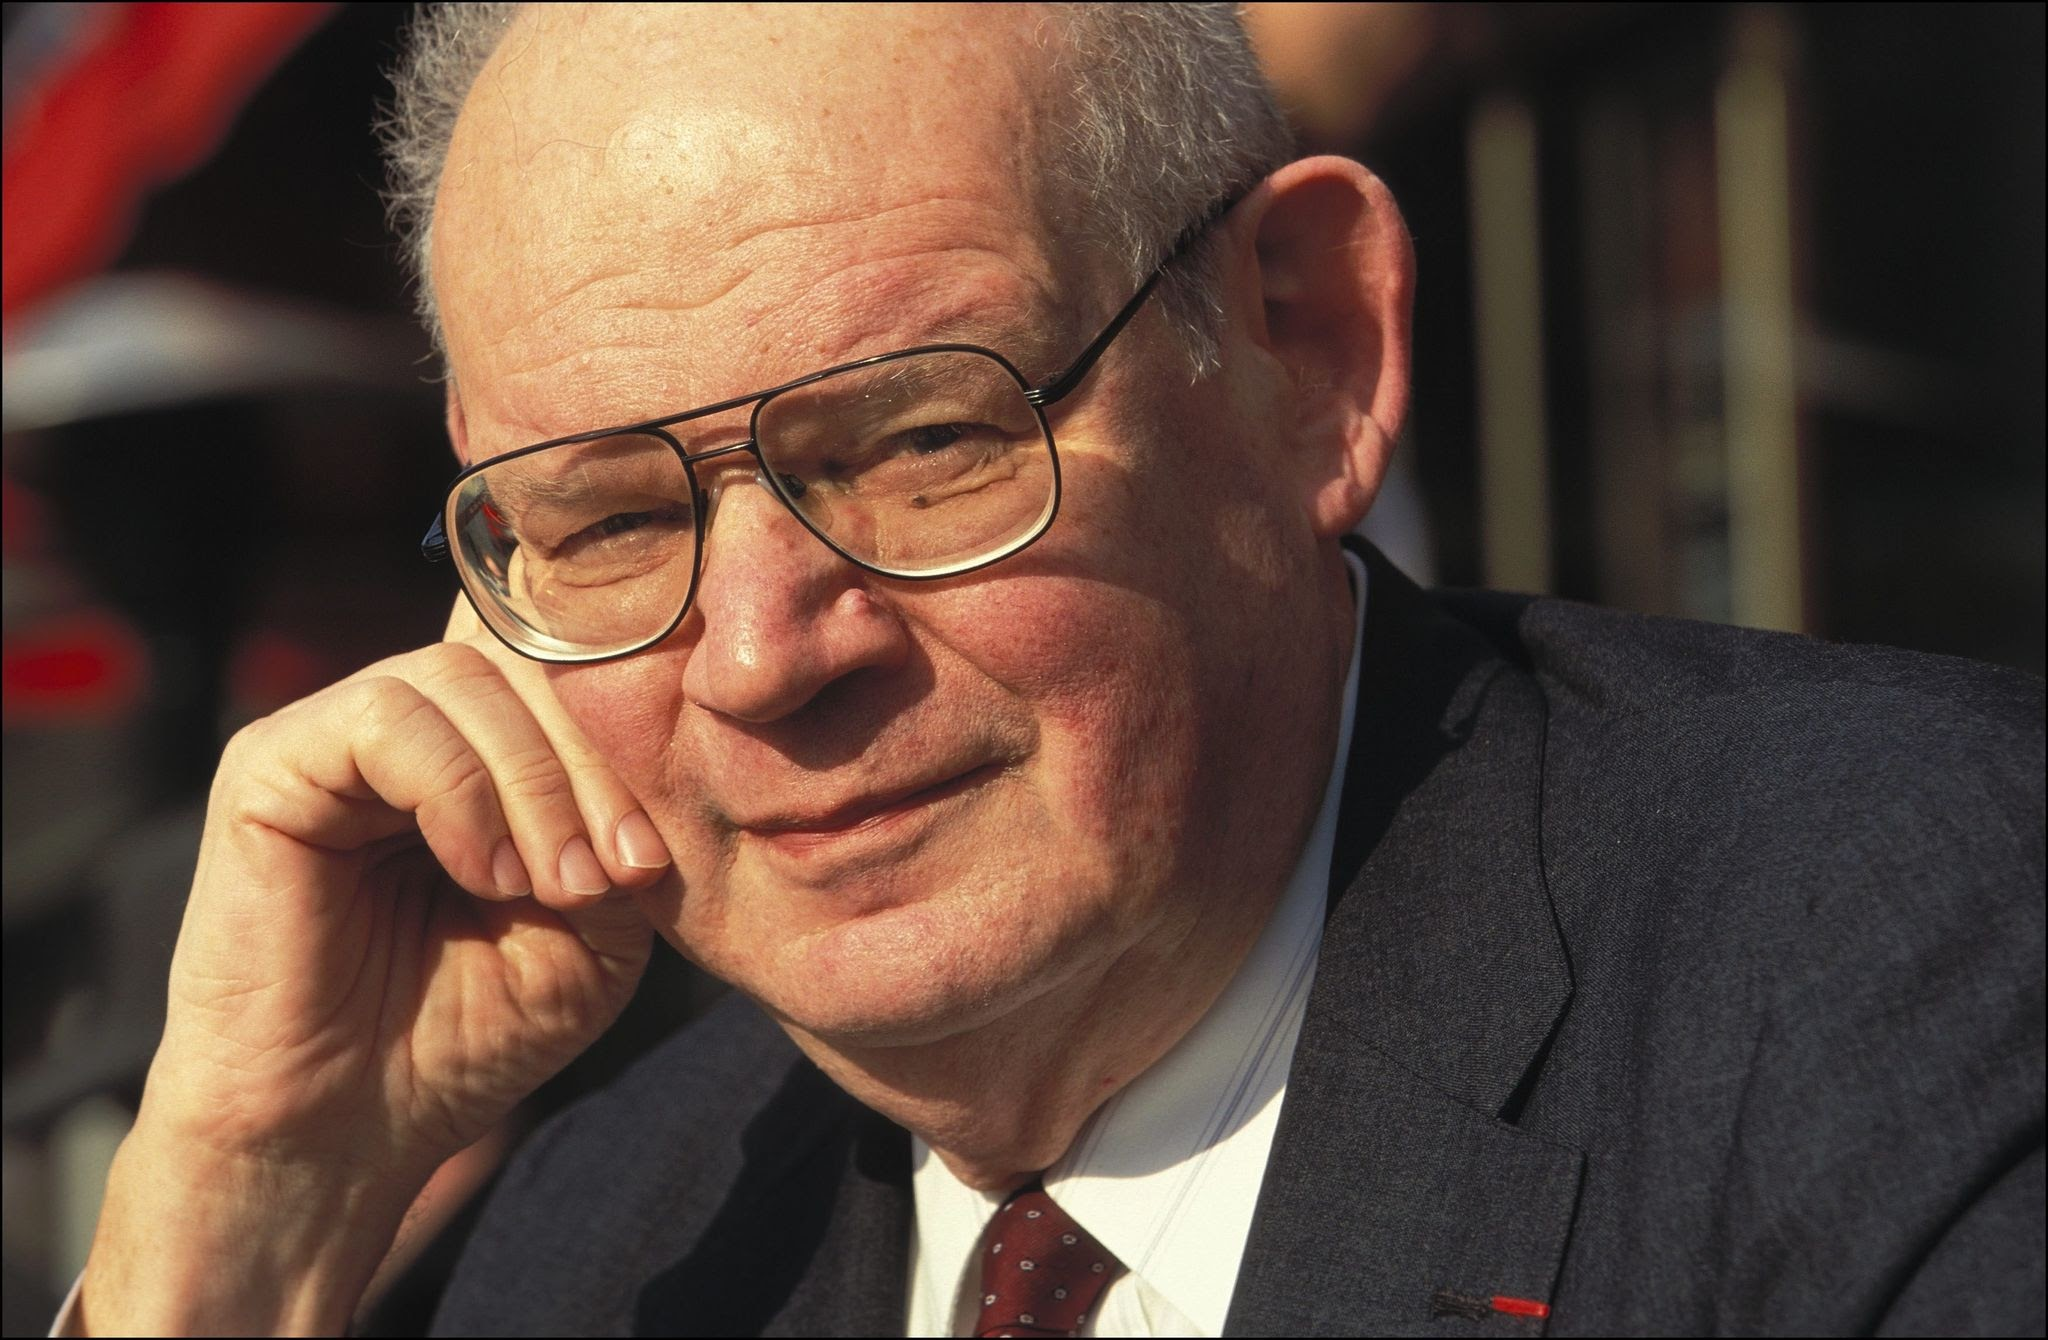
\includegraphics[width=\textwidth]{images/benoit-mandelbrot}
  \caption{Benoît Mandelbrot 1997 in Frankreich~\cite{gaillarde_benoit_1997}}
\end{center}
\end{figure}